\section{Coherent states}\label{sec:coherent-states}

\subsection{Summary of quadrature operators}

\hl{A coherent state is a linear superposition of number states} and this provides the closest approximation of a radiation by a laser. 

We already learned the relationship between the quadrature operators and the creation and annihilation operators:
\begin{equation}\label{eqn:13-quadratures-creation-annihilation-operators}
\begin{cases}
    \hat{x}_1 = \frac{1}{2}\, (\hat{a}+\hat{a}^\dagger ) \\
    \hat{x}_2 = \frac{i}{2}\, (\hat{a}-\hat{a}^\dagger ) 
\end{cases} \implies \hspace{2ex} \begin{cases}
    \hat{a} \hspace{0.23cm} = \hat{x}_1+i\hat{x}_2\\
    \hat{a}^\dagger  = \hat{x}_1-i\hat{x}_2
\end{cases}
\end{equation}

We are then allowed to write the Hamiltonian in terms of the quadrature operators:
\begin{equation}\label{eqn:13-hamiltonian-quadratures}
\hat{H} = \hbar \omega \left(\hat{a}^\dagger \hat{a}+\frac{1}{2}\right) =
\hbar \omega \left(\hat{x}_1^2+\hat{x}_2^2\right).
\end{equation}

We want to relay on photon number state, the basis can be used for black body radiation and chaotic light too. Remember that we have:
\begin{equation}\label{eqn:13-number-operator-eigenvalue-equation}
\hat{n}\,\ket{n} = n\, \ket{n},
\end{equation}

with uncertainty
\begin{equation}\label{eqn:13-number-operator-uncertainty}
\begin{split}
\braket{\Delta n^2} &= \braket{\hat{n}^2} - \braket{\hat{n}}^2 =\\[0.5ex]
&= \braket{n|\hat{n}\, \hat{n}|n}-(\braket{n|\hat{n}|n})^2 = \\[0.5ex]
&= n^2-n^2 = 0
\end{split}
\end{equation}

and we can write the Hamiltonian eigenvalue equation both in terms of the number operator and the quadrature operators:
\begin{equation}\label{eqn:13-hamiltonian-eigenvalue-equation}
\hat{H}\, \ket{n} = \hbar \omega \left(\hat{a}^\dagger \hat{a}+\frac{1}{2} \right)\, \ket{n} =\hbar \omega \bigl(n+\frac{1}{2}\bigr) = \hbar \omega \left(\hat{x}_1^2+\hat{x}_2^2\right)\, \ket{n}
\end{equation}

simplifying:
\begin{equation}
\left(\hat{x}_1^2+\hat{x}_2^2\right)\, \ket{n} = \left(n+\frac{1}{2}\right) \, \ket{n}
\end{equation}
\vspace{1ex}

Since the expectation values of the quadrature operators are zero $\braket{n|\hat{x}_1|n} = \braket{n|\hat{x}_2|n} = 0$, if we define the rotated quadrature operator as:
\begin{equation}\label{eqn:13-rotated-quadrature-operator}
X_\theta = \cos(\theta)\, \hat{x}_1+\sin(\theta) \, \hat{x}_2
\end{equation}

it will also have zero expectation value $\braket{n|X|n} = 0$ for any phase $\theta$. This means that the average value of the electric field is zero in a number state, and the phase is completely undefined.

A photon number state $\ket{n}$ represents an exotic state of light in sharp contrast with a classical electromagnetic wave of stable amplitude and phase. While a Fock state possesses a perfectly sharp energy (and photon number), it does not possess a classical phase analogue. In fact, a state $\ket{n}$ has a completely random phase, whereas a state with a well-defined phase must exhibit a completely broad photon number distribution. This highlights that quantum phase and photon number are complementary observables, obeying a fundamental uncertainty relation similar to position and momentum.

The vacuum state $\ket{0}$ for a single mode of frequency $\omega$ acts as the effective ground state of the system when thermal fluctuations are negligible, namely when the thermal energy is much smaller than the quantum excitation energy:
\begin{equation}\label{eqn:13-vacuum-thermal-condition}
k_B T \ll \hbar \omega.
\end{equation}

While the first excited state $\ket{1}$ (a single photon) can be generated experimentally via atomic cascade emissions or through spontaneous parametric down-conversion (SPDC), higher excited states $\ket{2}, \ket{3}, \dots$ become increasingly challenging to prepare in the laboratory.

\subsubsection{Coherent States Formalism}

A single-mode laser light operating well above threshold possesses a well-defined, stable phase. Such classical-like radiation cannot be described by a single Fock state, but corresponds to a specific linear superposition known as a \textbf{coherent state}, denoted as $\ket{\alpha}$.

Classically, we can visualize a mode being excited by an external source that shifts the electric field from zero to a finite classical amplitude $\vec{E} \propto |\alpha| \neq 0$, which in turn drives the magnetic field, generating a self-propagating harmonic wave. In the quantum framework, this process is modeled by displacing the vacuum state away from the origin of the phase space to induce an oscillating expectation value for the field.

To formalize this, we introduce the unitary \textbf{displacement operator} $\hat{D}(\alpha)$, which shifts the vacuum state by a complex amplitude $\alpha \in \mathbb{C}$:
\begin{equation}\label{eqn:13-displacement-operator-definition}
\ket{\alpha} = \hat{D}(\alpha) \ket{0}.
\end{equation}

The displacement operator is generated by the creation and annihilation operators:
\begin{equation}\label{eqn:13-displacement-operator-exponential}
\hat{D}(\alpha) = e^{\alpha \hat{a}^\dagger  - \alpha^* \hat{a}}.
\end{equation}

From its definition and the Baker-Campbell-Hausdorff lemma, $\hat{D}(\alpha)$ satisfies the following fundamental properties:
\begin{align}
\hat{D}^\dagger (\alpha) &= \hat{D}^{-1}(\alpha) = \hat{D}(-\alpha), \label{eqn:13-displacement-property-1} \\
\hat{D}^\dagger (\alpha) \hat{a} \hat{D}(\alpha) &= \hat{a} + \alpha, \label{eqn:13-displacement-property-2} \\
\hat{D}^\dagger (\alpha) \hat{a}^\dagger  \hat{D}(\alpha) &= \hat{a}^\dagger  + \alpha^*. \label{eqn:13-displacement-property-3}
\end{align}

A crucial property of the coherent state $\ket{\alpha}$ is that it is a right eigenstate of the annihilation operator $\hat{a}$. This can be proven by inserting the identity operator $\mathbb{I} = \hat{D}(\alpha)\hat{D}^\dagger (\alpha)$:
\begin{align}
\hat{D}^\dagger (\alpha) \hat{a} \ket{\alpha} &= \hat{D}^\dagger (\alpha) \hat{a} \hat{D}(\alpha) \ket{0} \nonumber \\
&= (\hat{a} + \alpha) \ket{0} = 0 + \alpha \ket{0}. \label{eqn:13-proof-eigenvalue-step1}
\end{align}

Multiplying both sides from the left by $\hat{D}(\alpha)$, we immediately find:
\begin{equation}\label{eqn:13-coherent-eigenvalue}
\hat{a} \ket{\alpha} = \alpha \ket{\alpha}.
\end{equation}

Using this eigenvalue relation, the expectation value for the photon number operator $\hat{n} = \hat{a}^\dagger  \hat{a}$ in a coherent state is easily evaluated:
\begin{equation}\label{eqn:13-coherent-mean-photons}
\braket{\alpha|\hat{n}|\alpha} = \braket{\alpha|\hat{a}^\dagger  \hat{a}|\alpha} = \alpha^* \alpha \braket{\alpha|\alpha} = |\alpha|^2 = \overline{n}.
\end{equation}

Here, $\overline{n}$ represents the mean photon number, matching the energy intensity of a classical field. However, unlike a number state, a coherent state does not contain a sharp number of photons. It is composed of an infinite superposition of Fock states:
\begin{equation}\label{eqn:13-coherent-fock-expansion}
\ket{\alpha} = \sum_{n=0}^{\infty} \ket{n} \braket{n|\alpha}.
\end{equation}

By projecting the eigenvalue equation onto $\bra{n}$ and using the property $\bra{n}\hat{a} = \sqrt{n+1}\bra{n+1}$, one finds the recurrence relation that yields the expansion coefficients:
\begin{equation}\label{eqn:13-coherent-coefficients}
\braket{n|\alpha} = \frac{\alpha^n}{\sqrt{n!}} e^{-\frac{1}{2}|\alpha|^2} \quad \implies \quad \ket{\alpha} = e^{-\frac{1}{2}|\alpha|^2} \sum_{n=0}^{\infty} \frac{\alpha^n}{\sqrt{n!}} \ket{n}.
\end{equation}

It is important to note that distinct coherent states are not orthogonal, as they are projections of shifted wave-packets that overlap in phase space:
\begin{equation}\label{eqn:13-coherent-overlap}
\braket{\alpha_1|\alpha_2} = e^{-\frac{1}{2}|\alpha_1|^2 - \frac{1}{2}|\alpha_2|^2} \sum_{n=0}^{\infty} \frac{(\alpha_1^* \alpha_2)^n}{n!} = e^{-\frac{1}{2}|\alpha_1|^2 - \frac{1}{2}|\alpha_2|^2 + \alpha_1^* \alpha_2}.
\end{equation}

The physical overlap probability (the profile indistinguishability) is given by the absolute square:
\begin{equation}\label{eqn:13-coherent-overlap-squared}
|\braket{\alpha_1|\alpha_2}|^2 = e^{-|\alpha_1 - \alpha_2|^2}.
\end{equation}

Hence, coherent states are only approximately orthogonal when their complex amplitudes are significantly different, i.e., when $|\alpha_1 - \alpha_2| \gg 1$.

To compute the variance of the photon number, $(\Delta n)^2 = \braket{\hat{n}^2} - \overline{n}^2$, we expand the operator $\hat{n}^2$ using the commutation relation $[\hat{a}, \hat{a}^\dagger ] = 1$ to reorder it into a normal-ordered form:
\begin{equation}\label{eqn:13-normal-ordering-n2}
\hat{n}^2 = \hat{a}^\dagger  \hat{a} \hat{a}^\dagger  \hat{a} = \hat{a}^\dagger  ( \hat{a}^\dagger  \hat{a} + 1 ) \hat{a} = \hat{a}^\dagger  \hat{a}^\dagger  \hat{a} \hat{a} + \hat{a}^\dagger  \hat{a}.
\end{equation}
Taking the expectation value with respect to $\ket{\alpha}$ yields:
\begin{equation}\label{eqn:13-n2-expectation}
\braket{\alpha|\hat{n}^2|\alpha} = \braket{\alpha|\hat{a}^\dagger  \hat{a}^\dagger  \hat{a} \hat{a}|\alpha} + \braket{\alpha|\hat{a}^\dagger  \hat{a}|\alpha} = |\alpha|^4 + |\alpha|^2 = \overline{n}^2 + \overline{n}.
\end{equation}
Substituting this back into the variance definition, we obtain:
\begin{equation}\label{eqn:13-photon-variance-final}
(\Delta n)^2 = (\overline{n}^2 + \overline{n}) - \overline{n}^2 = \overline{n}.
\end{equation}

\hl{This identity, where the variance equals the mean ($(\Delta n)^2 = \overline{n}$), is the signature of a quantum \textbf{Poissonian process}}.

Indeed, the probability $P(n)$ of detecting exactly $n$ photons in a coherent state field matches the photon number distribution:
\begin{equation}\label{eqn:13-poisson-distribution}
P(n) = |\braket{n|\alpha}|^2 = \left| e^{-\frac{1}{2}|\alpha|^2} \frac{\alpha^n}{\sqrt{n!}} \right|^2 = e^{-|\alpha|^2} \frac{(|\alpha|^2)^n}{n!} = e^{-\overline{n}} \frac{\overline{n}^n}{n!}.
\end{equation}

This confirms that photocounting statistics of ideal laser light are fully governed by a Poisson distribution with mean intensity $\overline{n}$.

The fractional uncertainty in the number of photons in the coherent state is:
\[\frac{\Delta n}{\overline{n}} = \frac{\sqrt{\overline{n}}}{\overline{n}} =\frac{1}{\sqrt{\overline{n}}}\]
as a matter of course, it decreases with increase in the number mean photon $\overline{n}$.

\calloutinfo{%
The coherent states $\ket{\alpha}$ are quantum states close to the classical ones:
\begin{enumerate}
    \item The expectation value of the $\vec{E}$ has the form of a classical field;
    \item The fluctuations in the $\vec{E}$ variables are the same as for the vacuum;
    \item The fluctuations in the fractional uncertainty decreases with increasing the average photon number. This lead us to classical limit where variance of a stable wave vanishes.
    \item The states become well localized in phase with increasing of photon number.
\end{enumerate}
}

\callout{A coherent state can be represented with a phasor of length $|\alpha|$ and angle $\theta$.}{%
Since
\begin{equation}
\begin{cases}
    \hat{x}_1 = \sqrt{\tfrac{m\omega}{2\hbar}}\, \hat{q} =
    \frac{1}{2}(\hat{a}+\hat{a}^\dagger )\\
    \hat{x}_2 = \sqrt{2m\hbar \omega}\, \hat{p} = 
    \tfrac{1}{2i}(\hat{a}-\hat{a}^\dagger )
\end{cases}
\end{equation}

we shall write:
\begin{equation}\label{eqn:13-alpha-polar-form}
    \alpha = |\alpha|\, e^{i\theta}
\end{equation}
\begin{proof}
\begin{equation}\label{eqn:13-alpha-polar-form-proof}
    \begin{split}
    \braket{\alpha|\hat{x}_1|\alpha} = \frac{1}{2}\braket{\alpha|(\hat{a}^\dagger +\hat{a})|\alpha} = \frac{1}{2}(\alpha^*+\alpha) \\
    &\hspace{2.35cm}= \Re(\alpha) = |\alpha|\, \cos(\theta)\\\\
    \braket{\alpha|\hat{x}_2|\alpha} = \frac{1}{2}i\braket{\alpha|(\hat{a}^\dagger -\hat{a})|\alpha} = \frac{1}{2}(\alpha^*+\alpha) \\
    &\hspace{2.35cm}= \Im(\alpha) = |\alpha|\, \sin(\theta)\\
    \end{split}
\end{equation}
\end{proof}
}
\vspace{1ex}

If we use:
\[\begin{cases}
    \hat{x}_1^2 = \frac{1}{4}(\hat{a}^\dagger \hat{a}+2\hat{a}^\dagger \hat{a}+\hat{a}\hat{a}+1)\\[1ex]
    \hat{x}_2^2 = \frac{1}{4}(-\hat{a}^\dagger \hat{a}+2\hat{a}^\dagger \hat{a}-\hat{a}\hat{a}+1)
\end{cases}\]

It can be proven that:
\[(\Delta \hat{x}_1)^2 = (\Delta \hat{x}_2)^2 = \frac{1}{4}\]

In contrast to the variances for the number state, \hl{the coherent state is a \textbf{quadrature-minimum uncertainty state} for all mean photon numbers $\overline{n} =|\alpha|^2$}.
The mean field amplitude associated with the coherent state is an arrow of length $|\alpha| = \sqrt{\overline{n}}$ inclined at an angle $\theta$ to the real axis.
\begin{figure}[H]
        \centering
        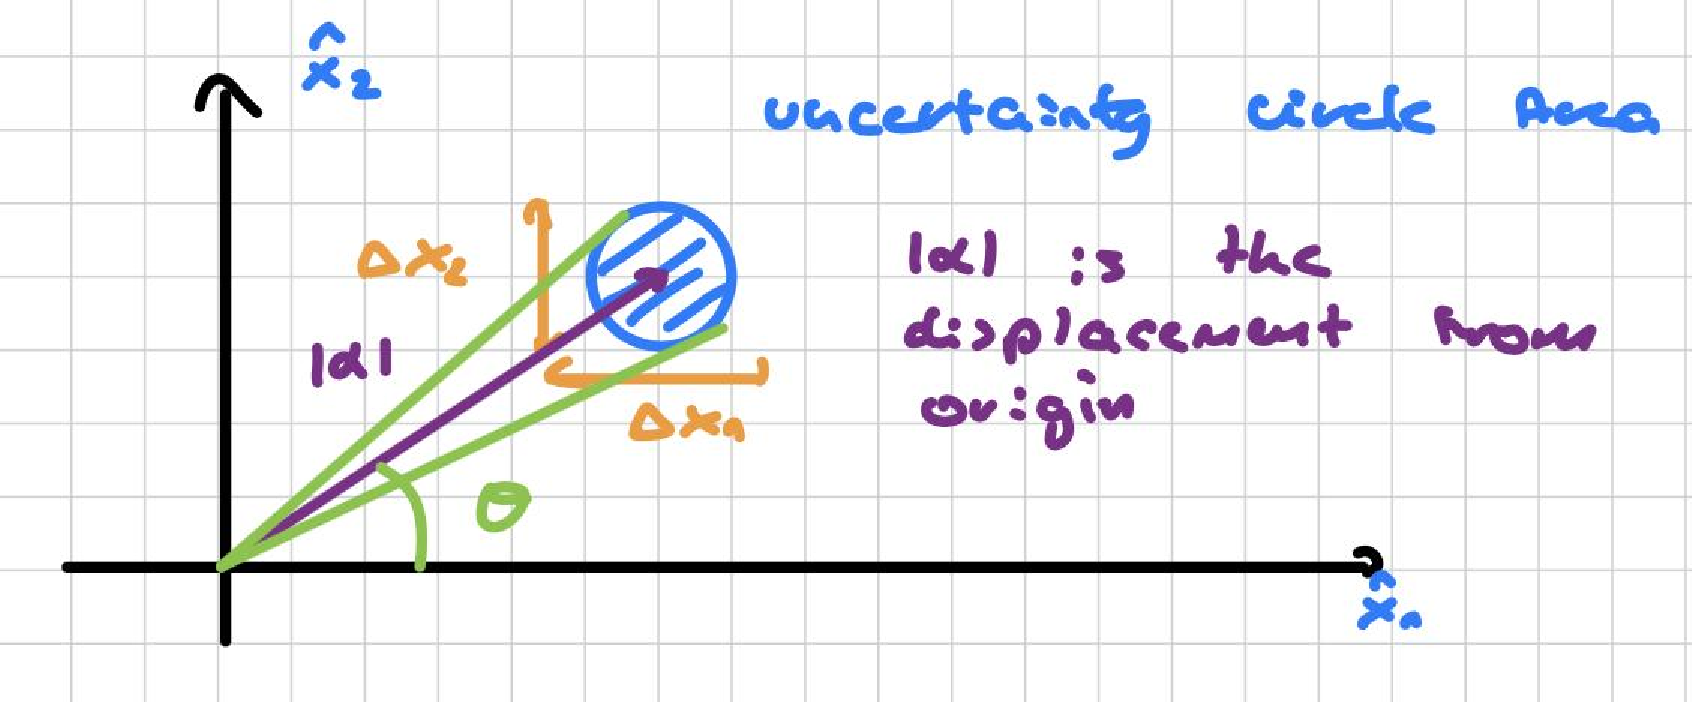
\includegraphics[width=0.6\linewidth]{images_in_pdf/13-/Grafico_68.pdf}
    \end{figure}

$|\alpha|^2$ and $\theta$ are uncertain, in contrast with the classical wave where these quantities are well known.

The length of the phasor is between $\alpha+\frac{1}{4}$ and $\alpha-\frac{1}{4}$:
\[ 
\begin{split}
    \Delta n &= \bigl(\sqrt{\overline{n}}+\frac{1}{4}\bigr)^2-\bigl(\sqrt{\overline{n}}-\frac{1}{4}\bigr)^2 \\
    &=\bigl(|\alpha|+\frac{1}{4}\bigr)^2-\bigl(|\alpha|-\frac{1}{4}\bigr)^2 \\
    &= |\alpha| = \sqrt{\overline{n}}
\end{split}
\]

\subsubsection{The shot-noise in optical detection is a result of quantum nature of light}

$\Delta \theta$ subtended by the diameter of the disk at origin. If $|\alpha| >> 1$ the arc rule gives:
\[\Delta\theta \approx \frac{\text{uncertainty diameter}}{|\alpha|} =\frac{\frac{1}{2}}{|\alpha|} = \frac{1}{2\sqrt{\overline{n}}}\]
We can calculate:
\[\Delta n \, \Delta \theta = \sqrt{\overline{n}}\, \frac{1}{2\sqrt{\overline{n}}} = \frac{1}{2}\]

This is a form of an uncertainty relation, but obtained by geometrical argument. So $\frac{\Delta \overline{n}}{\overline{n}}$ and $\Delta \theta$ vary like $\frac{1}{\alpha}$. When $\overline{n}$ increases, the E.M. waves becomes better defined both in amplitude and phase and lead us to the classical wave limit.

So what we see is:
\begin{itemize}
    \item \textbf{Coherent states $\ket{\alpha}$}:
    Fluctuation are equal in every direction (circle).
    \begin{figure}[H]
        \centering
        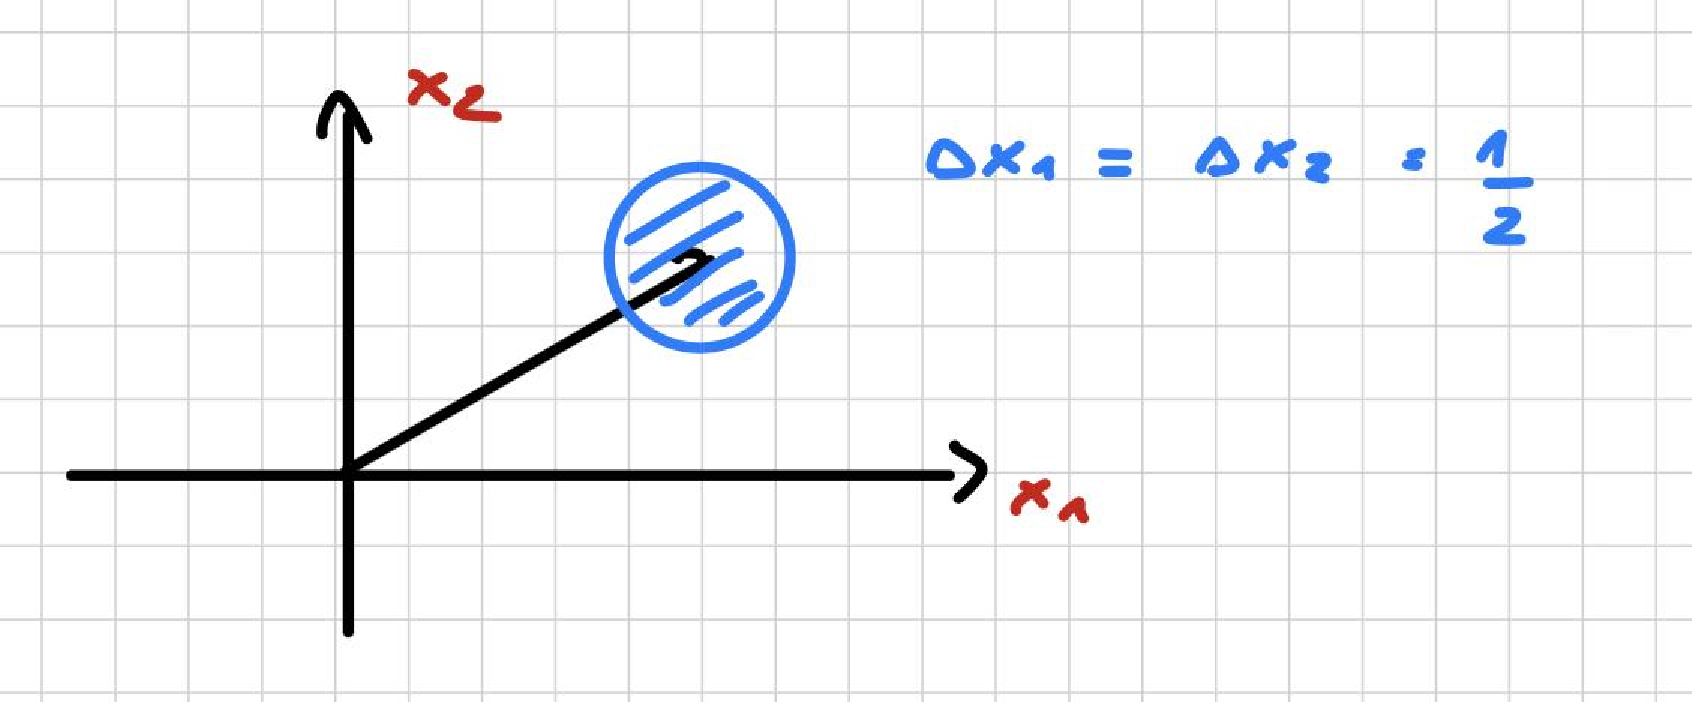
\includegraphics[width=0.6\linewidth]{images_in_pdf/13-/Grafico_69.pdf}
    \end{figure}

    Center is at distance $|\alpha| = \sqrt{\overline{n}}$ at angle $\theta$ above x-axis.
    
    \item \textbf{Vacuum state $\ket{0}$}: 
    Fluctuation are equal in every direction(circle.)
    \begin{figure}[H]
        \centering
        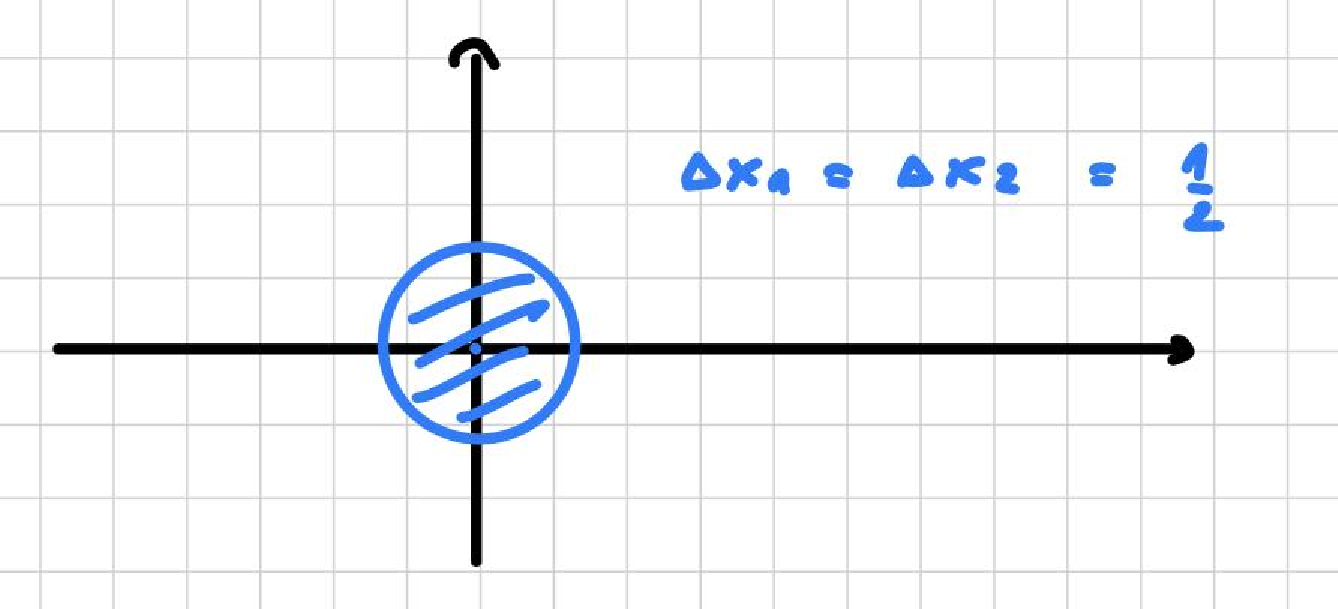
\includegraphics[width=0.6\linewidth]{images_in_pdf/13-/Grafico_70.pdf}
    \end{figure}

    $|\alpha |= 0$ and $\Delta \theta$ is large as possible $\Delta \theta = 2\pi$
    
    \textbf{Number state $\ket{n}$}: 
    We have a circle of radius $n$.
    \begin{figure}[H]
        \centering
        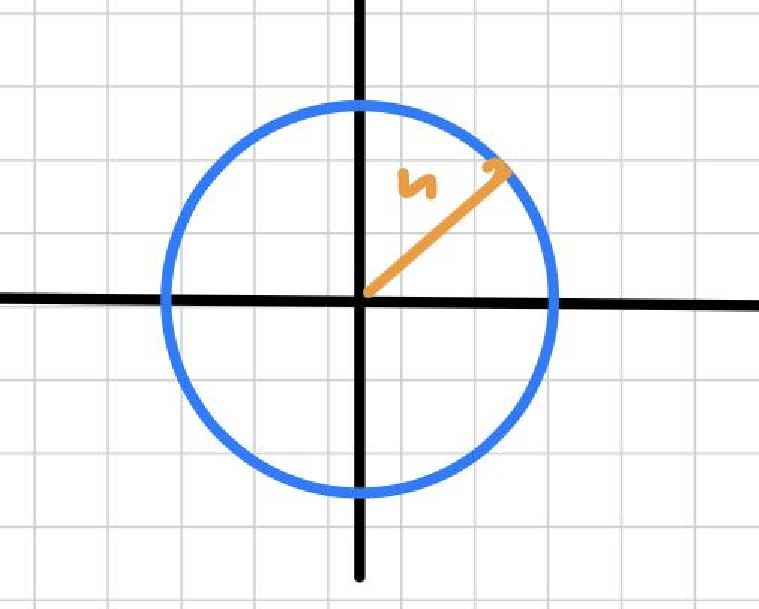
\includegraphics[width=0.6\linewidth]{images_in_pdf/13-/Grafico_71.pdf}
    \end{figure}

    $\Delta n = 0$, we know the number of photons, $\Delta \theta = 2\pi$  is max 
\end{itemize}
We recall the operator:
\[\begin{cases}
    \hat{E}_x =A_0 (\hat{a}+\hat{a}^\dagger )\sin(kz)\\
    \hat{x}_1 = \frac{1}{2}(\hat{a}+\hat{a}^\dagger ) 
\end{cases} \implies\hat{E}_x = 2A_0\, \sin(kz) \, \hat{x}_1 \]
Let us consider the time evolution of a quantum state for not interacting field:
\[\begin{split}
    &\ket{\alpha} \to \ket{\alpha e^{-i\omega t}}\\
    \implies &\bra{\alpha e^{-i\omega t}} \hat{x}_1 \ket{\alpha e^{-i\omega t}} = \alpha\,  \cos(\omega t)\\
    \implies &\bra{\alpha e^{-i\omega t}} \hat{x}_2 \ket{\alpha e^{-i\omega t}} = -\alpha\,  \sin(\omega t)\\
\end{split}\]
In the phasor diagram that means a clockwise rotation of the circle. 
\begin{figure}[H]
        \centering
        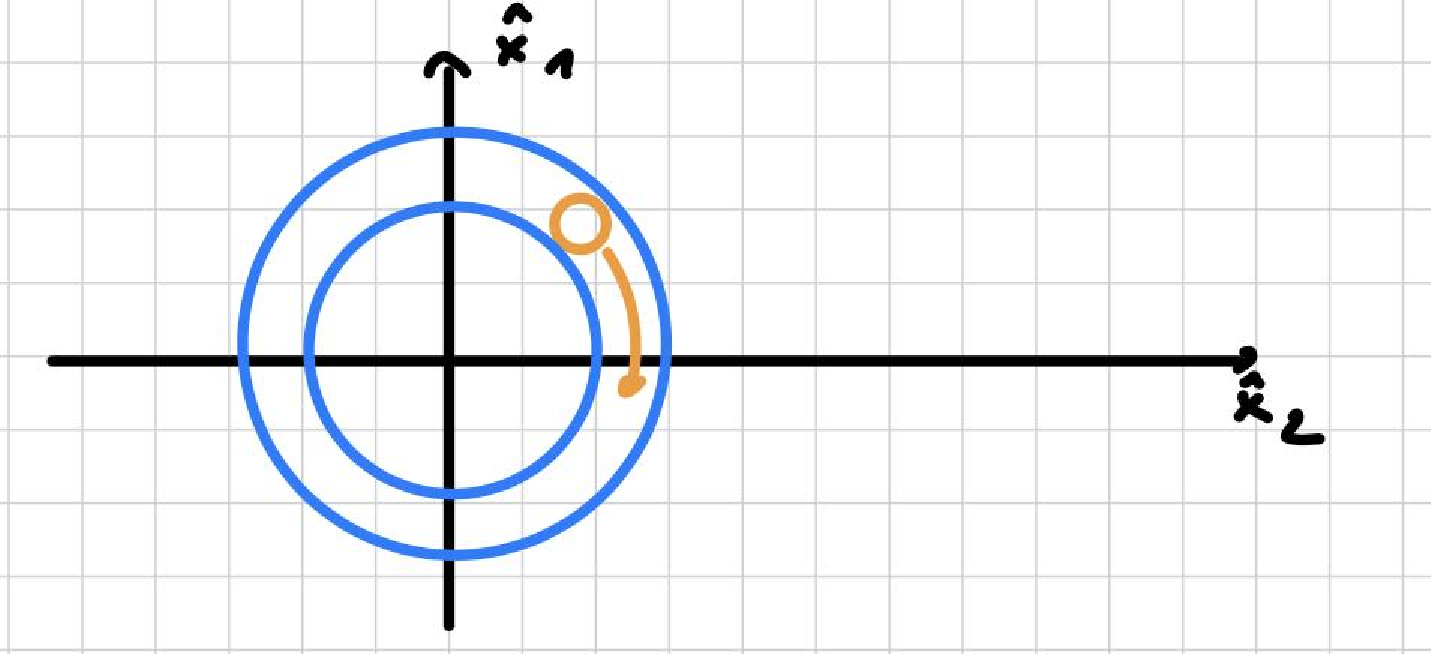
\includegraphics[width=0.6\linewidth]{images_in_pdf/13-/Grafico_72.pdf}
    \end{figure}

\[  \bra{\alpha e^{-i\omega t}} \hat{E}_x \ket{\alpha e^{-i\omega t}} = 2A_0\,  \sin(\omega t) \, \braket{\hat{x}_1} = 2A_0\,  \sin(\omega t) \, \alpha \, \cos(\omega t) \]
The time evolution is the projection of the $\braket{\hat{x}_1}$ axis as a function of the time.
\begin{figure}[H]
    \centering
    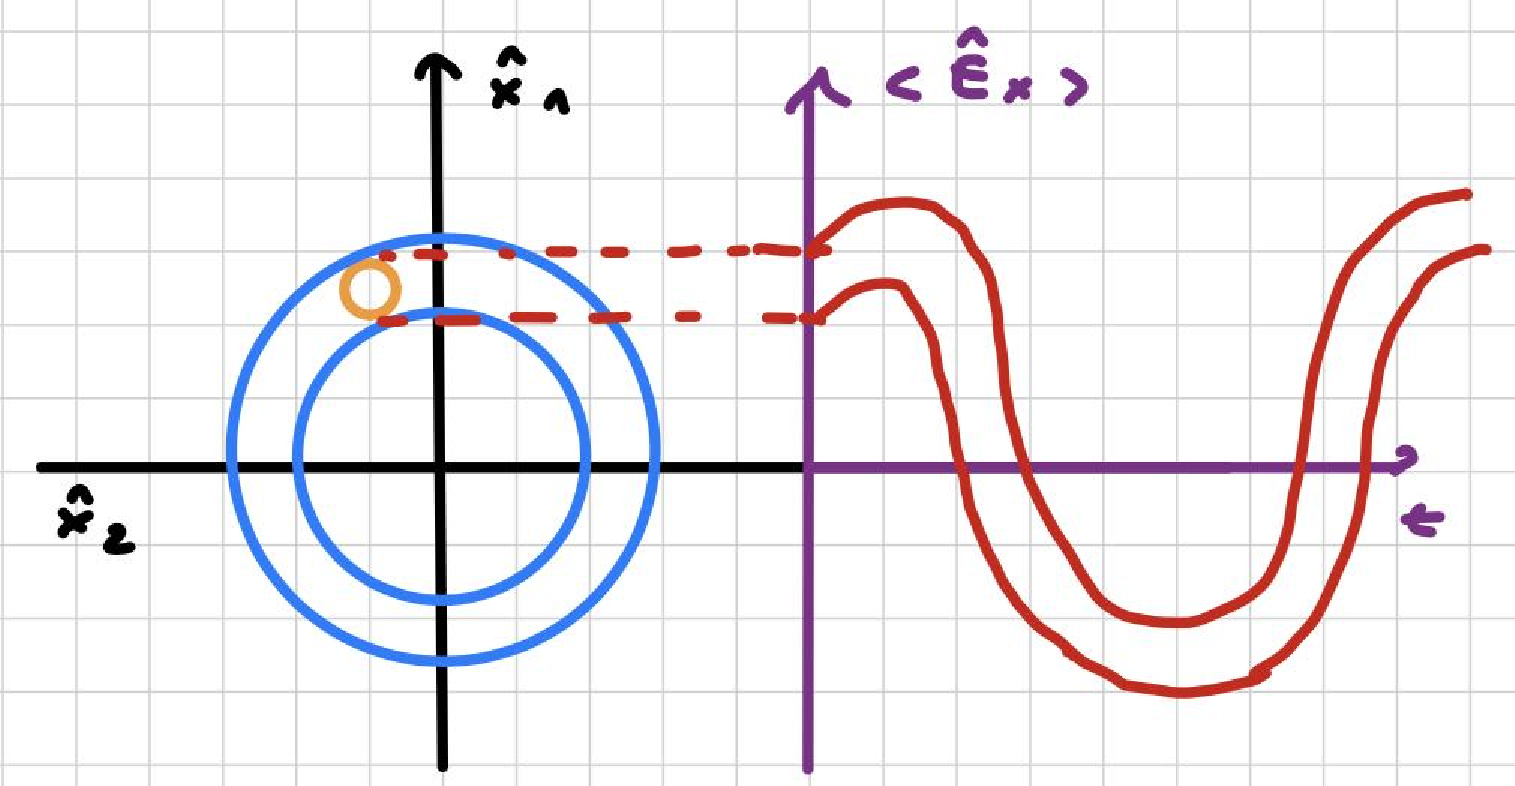
\includegraphics[width=0.6\linewidth]{images_in_pdf/13-/Grafico_73.pdf}
\end{figure}

Notice that the greater is the field $\braket{\hat{E}_x} \propto \alpha$, more the field appears classical. Coherent state is the most classical of all the quantum states, the expectation value of field must be very different from the classical ones. In case of number state $\braket{\hat{E}_x} = $.  However we will see that there are states with expectation value different from zero, but the fluctuations are less than a coherent state in one part of the field. These kind of states are called $\textbf{SQUEEZED STATES}$.

\subsubsection{Squeezed states}

We have other minimum uncertainty states with: 
\[\Delta x_1^2 < \frac{1}{4} \hspace{1cm} \text{or} \hspace{1cm} \Delta x_2^2 > \frac{1}{4}\]
This means that we have less noise in one of the quadrature operators, the circle is \textbf{squeezed} into an ellipse of the same area: 
\begin{figure}[H]
        \centering
        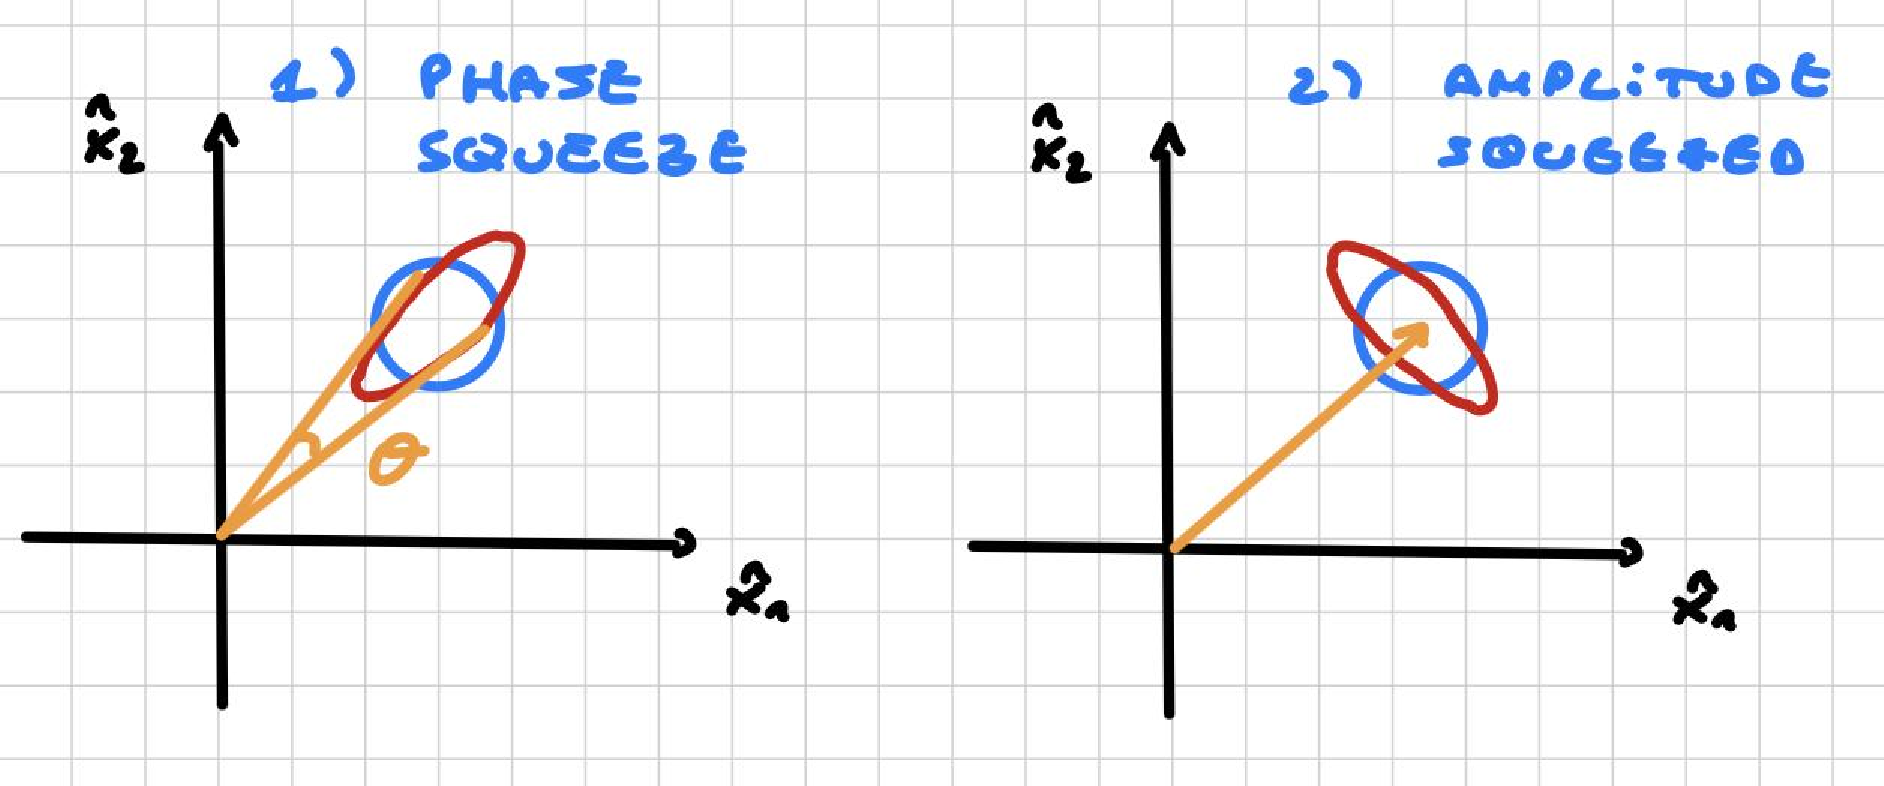
\includegraphics[width=0.6\linewidth]{images_in_pdf/13-/Grafico_74.pdf}
    \end{figure}

While coherent state have poissonian photon number distribution and shot-noise, \textbf{the amplitude-squeezed light will have sub-poissonian statistics with a noise level below the shot-noise.}

These states are represented by $(\alpha,\epsilon)$ with $\epsilon = r_s \, e^{i2\theta_s}$, where:
\begin{itemize}
    \item $|\alpha|^2$ is the intensity of the state.
    \item $\theta_s$ is the orientation of the squeezing axis.
    \item$r_s$ is the degree of squeezing, $\epsilon = 0$ for a coherent state.
\end{itemize}

We can generate a squeezed state starting from a vacuum state:
\[ \ket{\alpha,\epsilon} = \hat{D}(\alpha) \, \hat{S}(\epsilon) \, \ket{0}\]
Where we define the \textbf{squeezing operator}:
\begin{equation}\label{eqn:13-squeezing-operator}
    \hat{S}(\epsilon) = 
    \exp{
        \left(
            \frac{1}{2}\epsilon^*\hat{a}^2-\frac{1}{2}\epsilon \hat{a}^\dagger 
        \right)}
\end{equation}

We can compute:
\begin{align}\label{eqn:13-squeezed-state-expectation-values}
    &\bra{\alpha,\epsilon} \hat{a} \ket{\alpha,\epsilon} = \alpha\\[0.5ex]
    &\bra{\alpha,\epsilon} \hat{a}^2 \ket{\alpha,\epsilon} = \alpha^2-\cosh(r_s)\, \sinh(r_s)\, e^{2i\theta_s}\\[0.5ex]
    &\bra{\alpha,\epsilon} \hat{a}^\dagger \hat{a} \ket{\alpha,\epsilon} = |\alpha|^2+\sinh^2(r_s)
\end{align}

The coherent state are obtained for $r_s \to 0$, while the vacuum states are obtained for $\alpha \to 0$.

We can define the rotated quadrature operators for vacuum state:
\begin{equation}\label{eqn:13-rotated-quadrature-operator-squeezed}
\left(
\begin{matrix}
    \hat{y}_1\\[0.5ex]
    \hat{y_2}
\end{matrix}
\right) = 
\left(
\begin{matrix}
    \cos (\tfrac{\theta}{2}) &\sin(\tfrac{\theta}{2})\\[0.5ex]
    -\sin(\tfrac{\theta}{2}) &\cos(\tfrac{\theta}{2})
\end{matrix} 
\right)
\, 
\left(
\begin{matrix}
    \hat{x}_1\\[0.5ex]
    \hat{x}_2
\end{matrix}
\right)
\end{equation}

Or:
\[\hat{y}_1+i\hat{y}_2 = (\hat{x}_1+\hat{x}_2)\, e^{-i\frac{\theta}{2}}\]
The variances should be:
\[\begin{cases}
    \Delta \hat{y}_1^2 = \frac{1}{4}e^{-2r_s}\\[0.5ex]
    \Delta \hat{y}_2^2 = \frac{1}{4}e^{+2r_s}
\end{cases}\]

\begin{figure}[H]
    \centering
    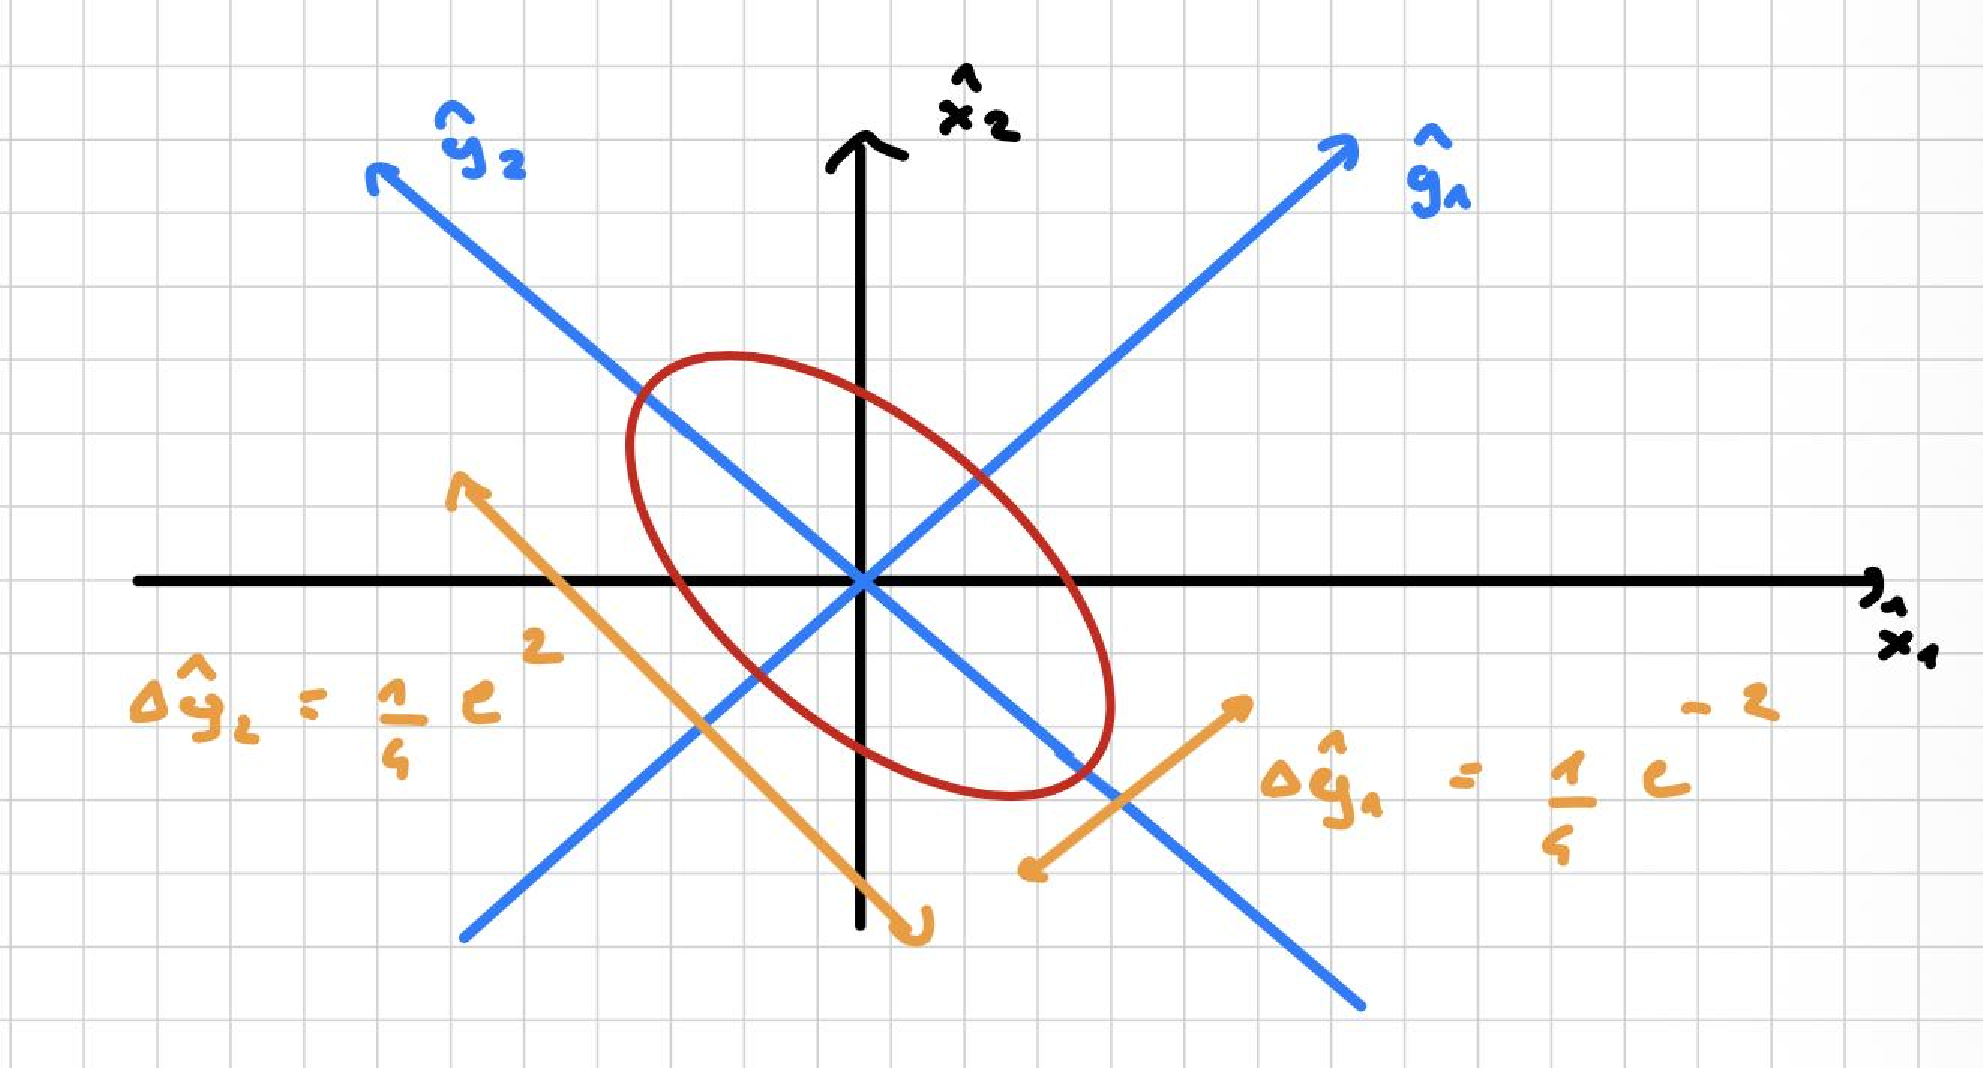
\includegraphics[width=0.6\linewidth]{images_in_pdf/13-/Grafico_75.pdf}
\end{figure}

For a generic squeeze state $\ket{\alpha,\epsilon}$, we have:
\[\braket{\hat{y}_1+i\hat{y}_2} = \alpha e^{-i\frac{\theta}{2}}\]
\begin{figure}[H]
        \centering
        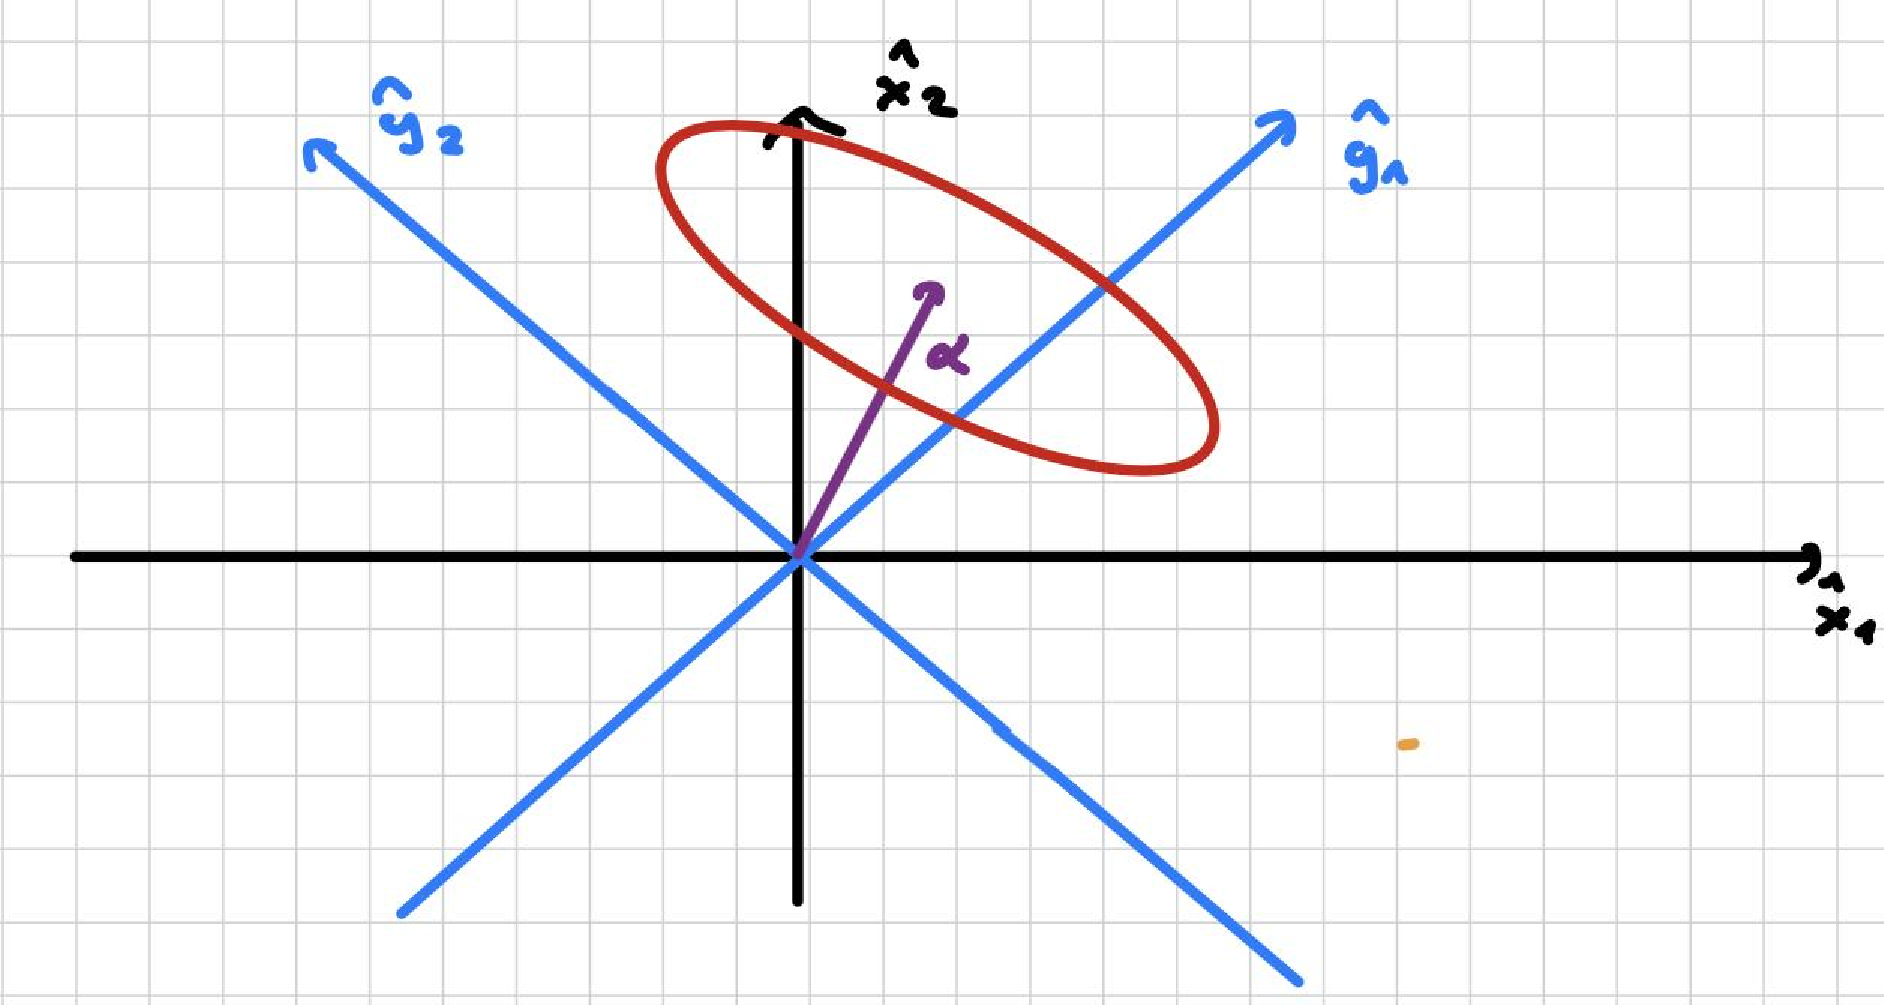
\includegraphics[width=0.6\linewidth]{images_in_pdf/13-/Grafico_76.pdf}
\end{figure}

Error ellipse is the same as for the squeeze vacuum, although displaced by $\alpha$. If we consider the single mode $\hat{E}$:
\[
\hat{E}(t) = A_0 \sin(kz)\bigl(\hat{a}e^{-i\omega t}+\hat{a}^\dagger e^{i\omega t}\bigr)
\]

Where: 
\begin{itemize}
    \item $\omega t = $ phase of the field.
    \item $\hat{a},\hat{a}^\dagger =$ operators at $t=0$. 
\end{itemize}

If we set $x = \omega t$ and look at the Equation~\ref{eqn:11-electric-field-quadrature-operators}:
\begin{equation*}
\hat{E}(x)= 2A_0\, \sin(kz) [\hat{x}_1\, \cos(x) + \hat{x}_2 \, \sin(x)]
\end{equation*}

From the fact that:
\begin{equation}\label{eqn:13-commutation-relation-quadratures}
\bigl[\hat{x}_1,\hat{x}_2\bigr] = \frac{i}{2}
\end{equation}

 we obtain:
\begin{equation}\label{eqn:13-commutation-relation-electric-field}
\left[\hat{E}(x=0) ,\hat{E}(x)\right] = i A_0^2 \, \sin^2(kz)\, \sin(x)
\end{equation}

\hl{Operators at different phases don't commute!}

\callout{Proof of the commutation relation between $\hat{E}(x=0)$ and $\hat{E}(x)$.}{%
\begin{proof}
Let's start by evaluating the field at $x=0$:
\begin{equation}\label{eqn:13-electric-field-x0}
\hat{E}(x=0) = 2 A_0 \sin(kz)\, \hat{x}_1
\end{equation}

Next, we compute the actual commutator:
\begin{equation}\label{eqn:13-electric-field-commutator-proof}
\begin{split}
\left[
    \hat{E}(0), \hat{E}(x)
\right] &= 
\left(2 A_0\, \sin(kz)\right)^2 
\bigl[
    \hat{x}_1, \hat{x}_1 \cos(x) + \hat{x}_2 \sin(x)
\bigr] = \\[0.5ex]
&= 4 A_0^2 \, \sin^2(kz)
\bigl[
    \hat{x}_1, \hat{x}_2 \sin(x)
\bigr] = \\[0.5ex]
&= 4 A_0^2 \, \sin^2(kz) \sin(x) \bigl[
    \hat{x}_1, \hat{x}_2
\bigr]
\end{split}
\end{equation}

where we have used the fact that $\hat{x}_1$ commutes with itself and that $\sin(x)$ is a scalar factor. Substituting the commutation relation in Eqn.~\ref{eqn:13-commutation-relation-quadratures} into the above expression, the result is proven.
\end{proof}
}

If the uncertainty in the field at $x=0$ is:
\[\Delta \hat{E}(0) < \frac{1}{\sqrt{2}}A_0\,|\sin(kz)\, \sin(x)|\]
Then at some other phases we must have:
\[\Delta \hat{E}(x) > \frac{1}{\sqrt{2}} A_0\, |\sin(kz)\, \sin(x)|\]

\calloutinfo{%
    Squeeze light contains phase-dependent noise that is reduced below that of the vacuum for some phases and enhanced above that of the vacuum for others.
}

Distribution of noise in the $\vec{E}$ for squeezed states is:
\begin{figure}[H]
        \centering
        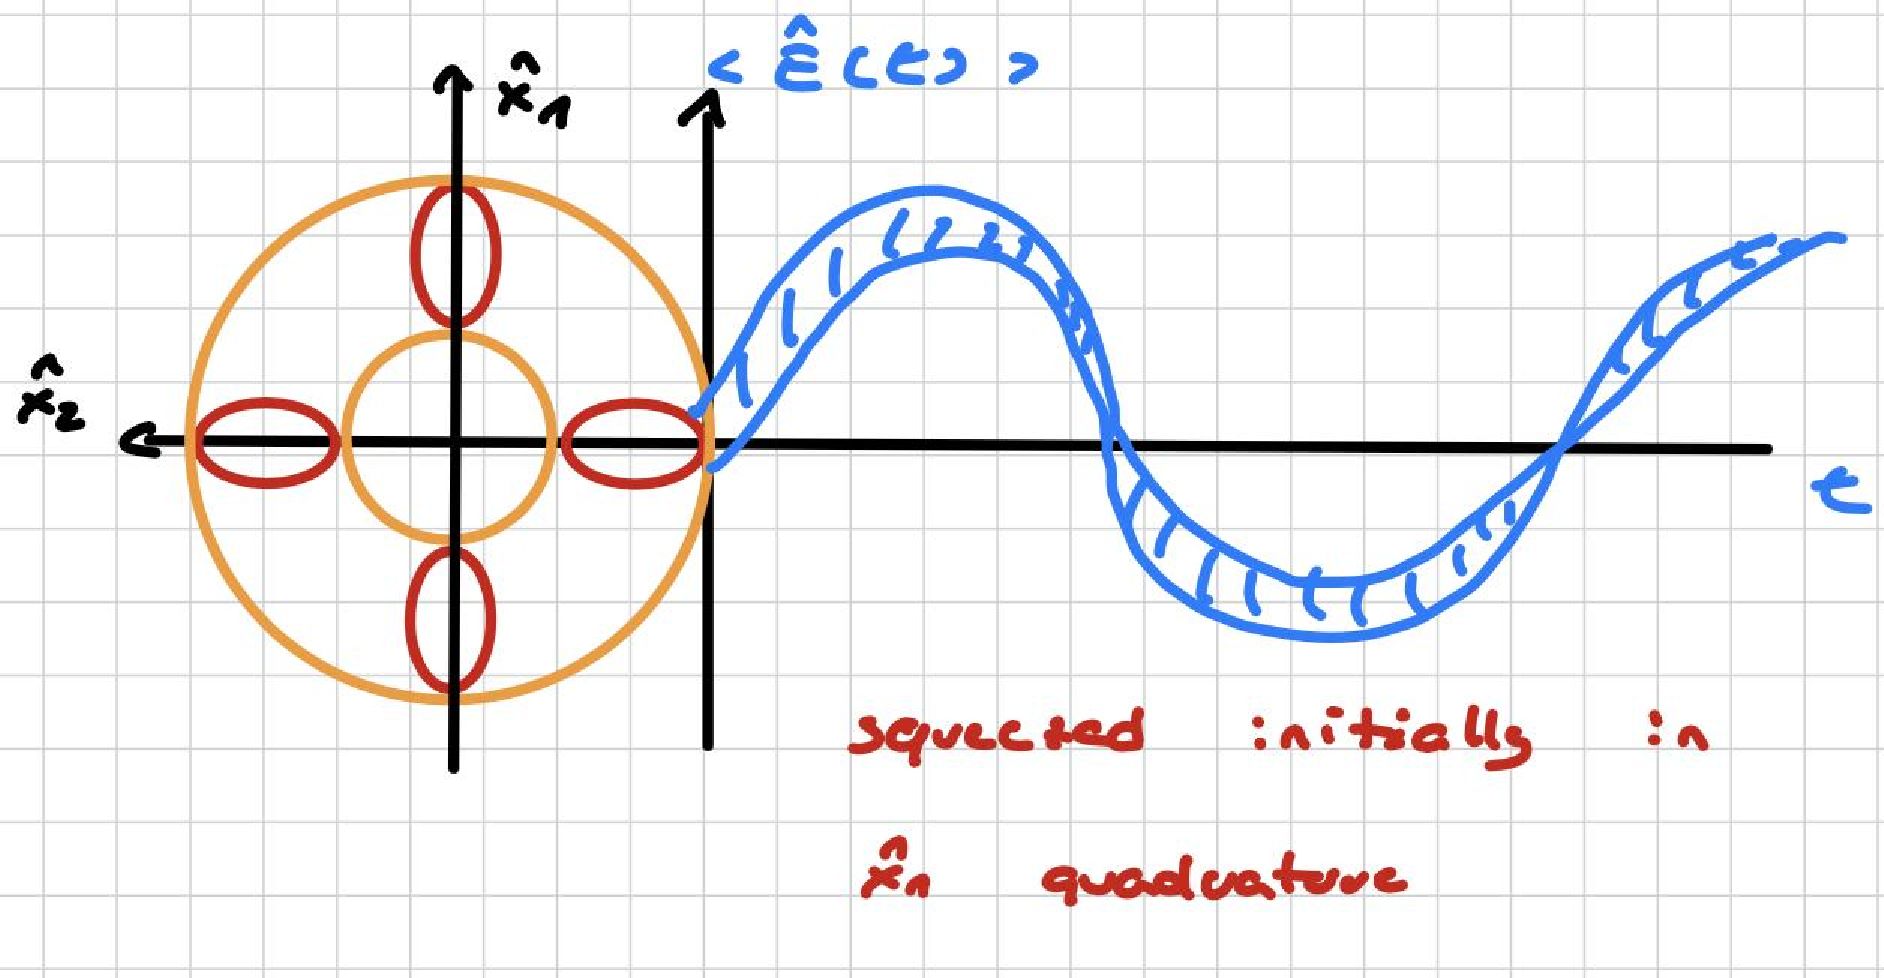
\includegraphics[width=0.6\linewidth]{images_in_pdf/13-/Grafico_77.pdf}
        \caption{}
    \end{figure}
\begin{figure}[H]
        \centering
        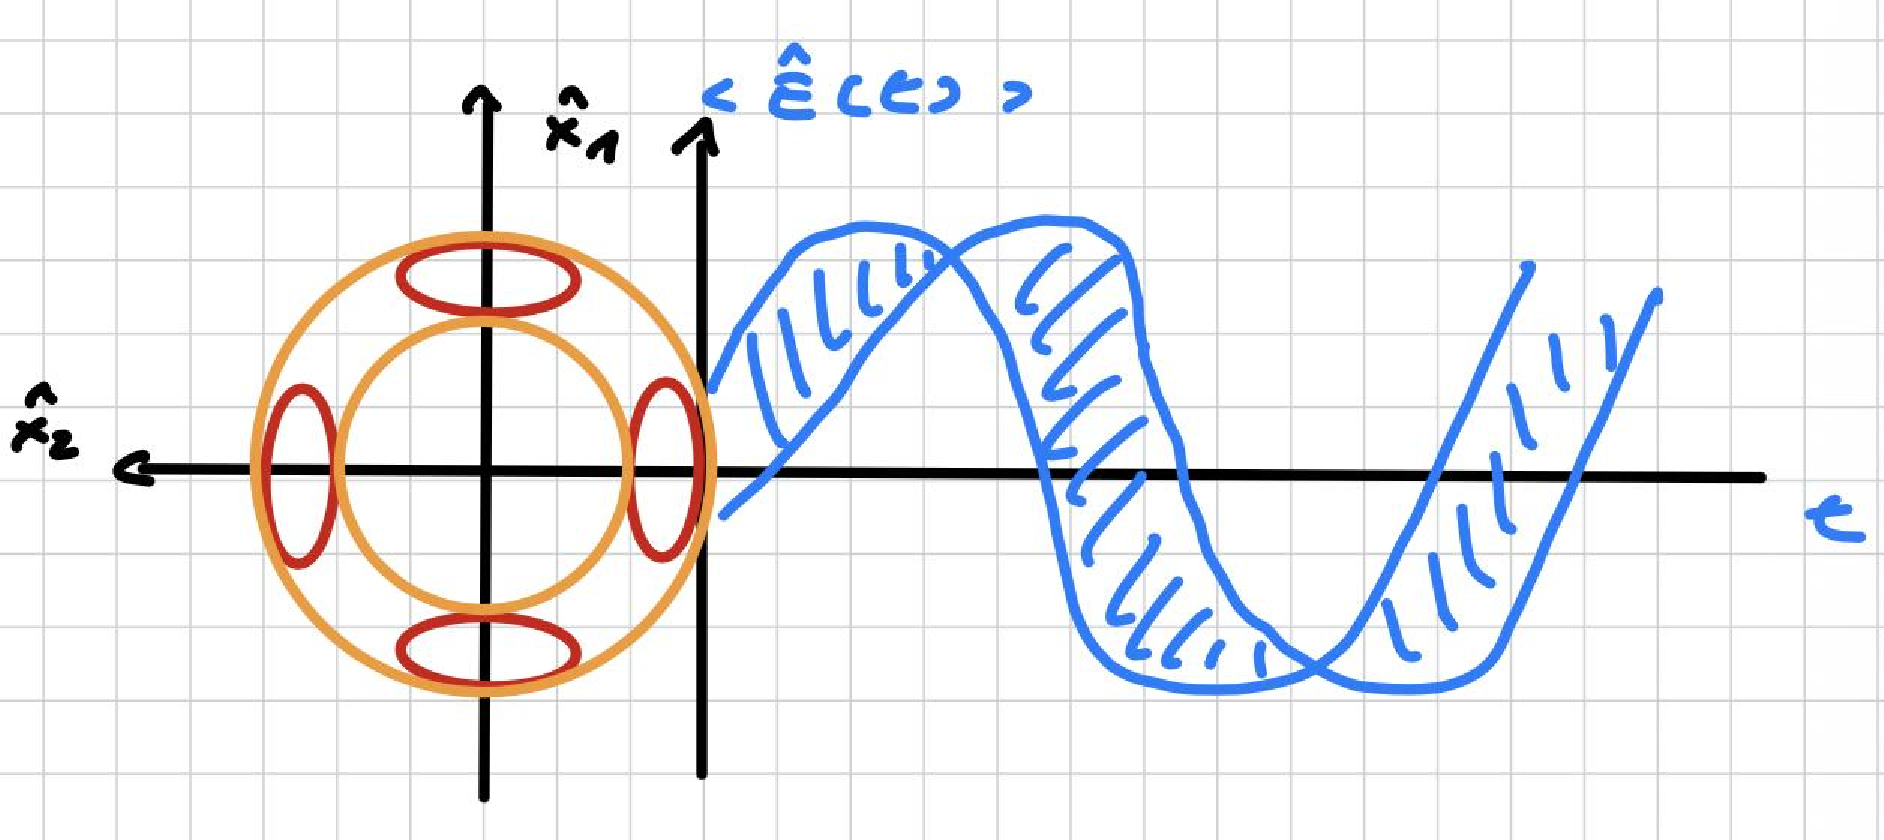
\includegraphics[width=0.6\linewidth]{images_in_pdf/13-/Grafico_78.pdf}
        \caption{}
    \end{figure}

It can be shown that:

\begin{table}[H]
\label{tab:squeezed-states}
  \centering
  \begin{tabular}{|c|c|c|}
    \hline
      & Amplitude squeezing &  Phase squeezing \\\\
    \hline
    $\Delta n$ & $\sqrt{\overline{n}}\cdot e^{-r_s}$ & $\sqrt{\overline{n}}\cdot e^{+r_s}$\\\\
    \hline
    $\Delta \theta$ & $\frac{1}{2\sqrt{\overline{n}}}\cdot e^{+r_s}$ & $\frac{1}{2\sqrt{\overline{n}}}\cdot e^{-r_s}$\\
  \end{tabular}
\end{table}

This means that $\Delta n_{A.S.} < \Delta n = \sqrt{\overline{n}}$ and $\Delta \theta_{P.S.} < \Delta \theta$, \textbf{the photon number fluctuation are sub-poissonian in a squeezed state.}